\documentclass[conference]{IEEEtran}

\usepackage[utf8]{inputenc}
\usepackage[T1]{fontenc}
\usepackage{mathptmx}
\usepackage[spanish,es-tabla,es-noshorthands,es-nolayout]{babel}
\addto\captionsspanish{\renewcommand{\figurename}{Fig.}\renewcommand{\refname}{Referencias}}
\usepackage{amsmath}
\usepackage{graphicx}
\usepackage{booktabs}
\usepackage{array}
\usepackage{textcomp}
\usepackage{cite}
\usepackage{url}
\usepackage{microtype}

\newcommand{\ohmm}{\ensuremath{\Omega\!\cdot\!\mathrm{m}}}
\graphicspath{{figs/}}
\hyphenation{Coapan Tehuac\'an}

\begin{document}
\renewcommand{\IEEEkeywordsname}{Palabras clave}

\title{Caracterizaci\'on geof\'isica propuesta del relleno sanitario de Santa Mar\'ia Coapan (Tehuac\'an, Puebla): dise\~no de campo e interpretaci\'on esperada}

\author{\IEEEauthorblockN{Ian A. Sandoval-Valderr\'abano \hspace{1.5em} Carlos Enrique Fern\'andez Tepale}
\IEEEauthorblockA{\textit{Facultad de Ingenier\'ia}\\
\textit{Benem\'erita Universidad Aut\'onoma de Puebla}\\
Puebla, M\'exico}}

\maketitle
\begin{abstract}
El relleno sanitario de Tehuacán, en la junta auxiliar de Santa María Coapan (Puebla), operó cerca de tres décadas. La comunidad y la organización Greenpeace afirman que recibió residuos peligrosos industriales y biológico-infecciosos. La PROFEPA ordenó su clausura total y definitiva el 27 de junio de 2023 y pidió un estudio del daño ambiental y un plan de remediación. Hasta donde se encontró en fuentes públicas, ese estudio no se ha presentado. Este trabajo propone cómo usar métodos geofísicos para responder tres preguntas que hoy no tienen respuesta medida: dónde están los residuos, hasta dónde llegó el lixiviado y si hay zonas con material metálico enterrado. Se diseña un levantamiento georreferenciado con tomografía de resistividad eléctrica (ERT) y polarización inducida (IP), electromagnético en el dominio de frecuencia (EM), magnetometría y radar de penetración terrestre (GPR), con piezómetros para confirmar. Para mostrar qué se espera ver, se simuló en 2.5D un perfil sintético de ERT (901 mediciones Wenner--Schlumberger, 3\,\% de ruido). La inversión ajustó con RMS de 3.5\,\%, recuperó bien el cuerpo de residuos (28 contra 30\,\ohmm\ del modelo) y ubicó el lixiviado, aunque lo suavizó y mostró más resistivo (17 contra 6\,\ohmm) extendiéndolo en profundidad. No hay mediciones geofísicas de campo: todo resultado del subsuelo es una predicción. En cambio, la ubicación real, las dimensiones (9.80\,ha de cuerpo principal y 12.15\,ha de huella operativa total en 18\textdegree24$'$17.53$''$N, 97\textdegree25$'$36.68$''$O) y la evolución superficial (1993--2025) sí se delimitaron mediante imágenes satelitales históricas y un modelo digital de elevación para georreferenciar el diseño propuesto.
\end{abstract}

\begin{IEEEkeywords}
geofísica ambiental, relleno sanitario, lixiviado, tomografía de resistividad eléctrica, polarización inducida, percepción remota, Tehuacán.
\end{IEEEkeywords}

\section{Introducción}
Un relleno sanitario bien diseñado aísla los residuos del suelo y del agua subterránea. Un tiradero sin control no lo hace: el agua de lluvia atraviesa los residuos y forma lixiviado, un líquido con sales, materia orgánica y, a veces, metales. Si ese líquido llega al acuífero, la contaminación se mueve bajo tierra sin que se vea en la superficie.

La geofísica ayuda en este problema porque el lixiviado conduce muy bien la electricidad. Por eso baja la resistividad del terreno, y la ERT puede dibujarlo desde la superficie sin excavar \cite{maurya2017,helene2020}. La polarización inducida (IP) agrega información sobre el tipo de material, por ejemplo, residuos con metales \cite{abdulrahman2016}.

El caso elegido es el relleno sanitario municipal de Tehuacán, en territorio de Santa María Coapan, Puebla. Es un problema ambiental real, tiene una resolución oficial de clausura y, según fuentes públicas, sigue sin estudio de daño ni remediación \cite{greenpeace,profepa}. Este informe no presenta mediciones geofísicas de campo; propone un proyecto de diseño respaldado por una delimitación satelital y topográfica real en \texttt{EPSG:32614} y muestra con una simulación numérica qué se espera resolver y qué no.

\section{Problemática a resolver}
\subsection{Qué pasó}
La Tabla~\ref{tab:cron} resume la historia del sitio. Las fuentes documentales no coinciden en el año de inicio (1993 o 1995), así que se reportan ambas fechas acotadas además por escenas Landsat históricas.

\begin{table}[!t]
\caption{Cronología del relleno sanitario de Tehuacán}
\label{tab:cron}
\centering
\small
\begin{tabular}{@{}p{0.2\columnwidth}p{0.72\columnwidth}@{}}
\toprule
Fecha & Hecho (fuente)\\
\midrule
1993--1995 & Inicio de operación: 1993 \cite{greenpeace}; junio de 1995, con 15 años de vida útil estimada \cite{linares}. Escenas Landsat muestran terreno intacto en feb. 1993 y obra abierta en dic. 1994 \cite{usgs}.\\
2010 & Año en que, según el proyecto original, debía dejar de operar \cite{linares}.\\
Oct. 2021 & La comunidad lo cierra de hecho (7 de octubre) \cite{greenpeace}.\\
Mayo 2022 & Incendio en el sitio (iniciado entre el 5 y 8 de mayo según Sentinel-2; cicatriz de 2.92\,ha). El Comité de Bienes afirma que borra evidencia \cite{ciudadano,esa}.\\
Jun. 2022 & La SMADSOT coloca sellos de clausura (nota del 13 de junio) \cite{publimetro}.\\
27 jun. 2023 & Resolución de la PROFEPA (Exp.\ PFPA/3.2/2C.27.1/00036-20): clausura total y definitiva; retirar residuos peligrosos y RPBI, estudiar el daño y presentar un plan de remediación \cite{greenpeace,profepa}.\\
\bottomrule
\end{tabular}
\end{table}

\subsection{Qué se dice y qué está comprobado}
Hay que separar los hechos documentados de las afirmaciones. La clausura de la PROFEPA y las fechas son documentadas \cite{greenpeace,profepa}. En cambio, lo siguiente son afirmaciones de la comunidad y de organizaciones, y este trabajo no las verifica: que se depositaron lodos industriales de lavanderías de mezclilla y residuos hospitalarios \cite{greenpeace,ciudadano}, que se acumularon 3.7 millones de toneladas \cite{greenpeace}, que el sitio creció 18\,ha dentro de la Reserva de la Biosfera Tehuacán-Cuicatlán \cite{ciudadano}, que hay filtración de lixiviados a la reserva y que hay casos de cáncer \cite{ciudadano,desinformemonos}.

Ninguna de esas cifras de volumen o salud viene de un estudio técnico independiente. En cambio, la evolución superficial sí puede medirse con imágenes satelitales: en junio de 2011 el núcleo consolidado medía 6.75\,ha (acorde con las 6--7.2\,ha autorizadas para el periodo original), en agosto de 2025 el cuerpo principal alcanzó 9.80\,ha ($\sim$10\,ha citadas en la tesis de Linares \cite{linares}) y la huella total perturbada suma 12.15\,ha al incluir un área auxiliar suroeste (2.11\,ha) y 0.24\,ha de franjas perimetrales de acceso y maniobra \cite{esri}. La diferencia respecto a las 16.46\,ha asignadas por la CONANP \cite{conanp} corresponde a franjas periféricas dentro de la subzona administrativa.

\subsection{Pregunta que se quiere responder}
\emph{¿Dónde están los residuos y el lixiviado en el subsuelo, hasta qué profundidad llegan y hacia dónde se mueven?} Sin esa respuesta física medida no es posible diseñar una remediación acorde con la resolución de la PROFEPA.

\begin{figure*}[!t]
\centering
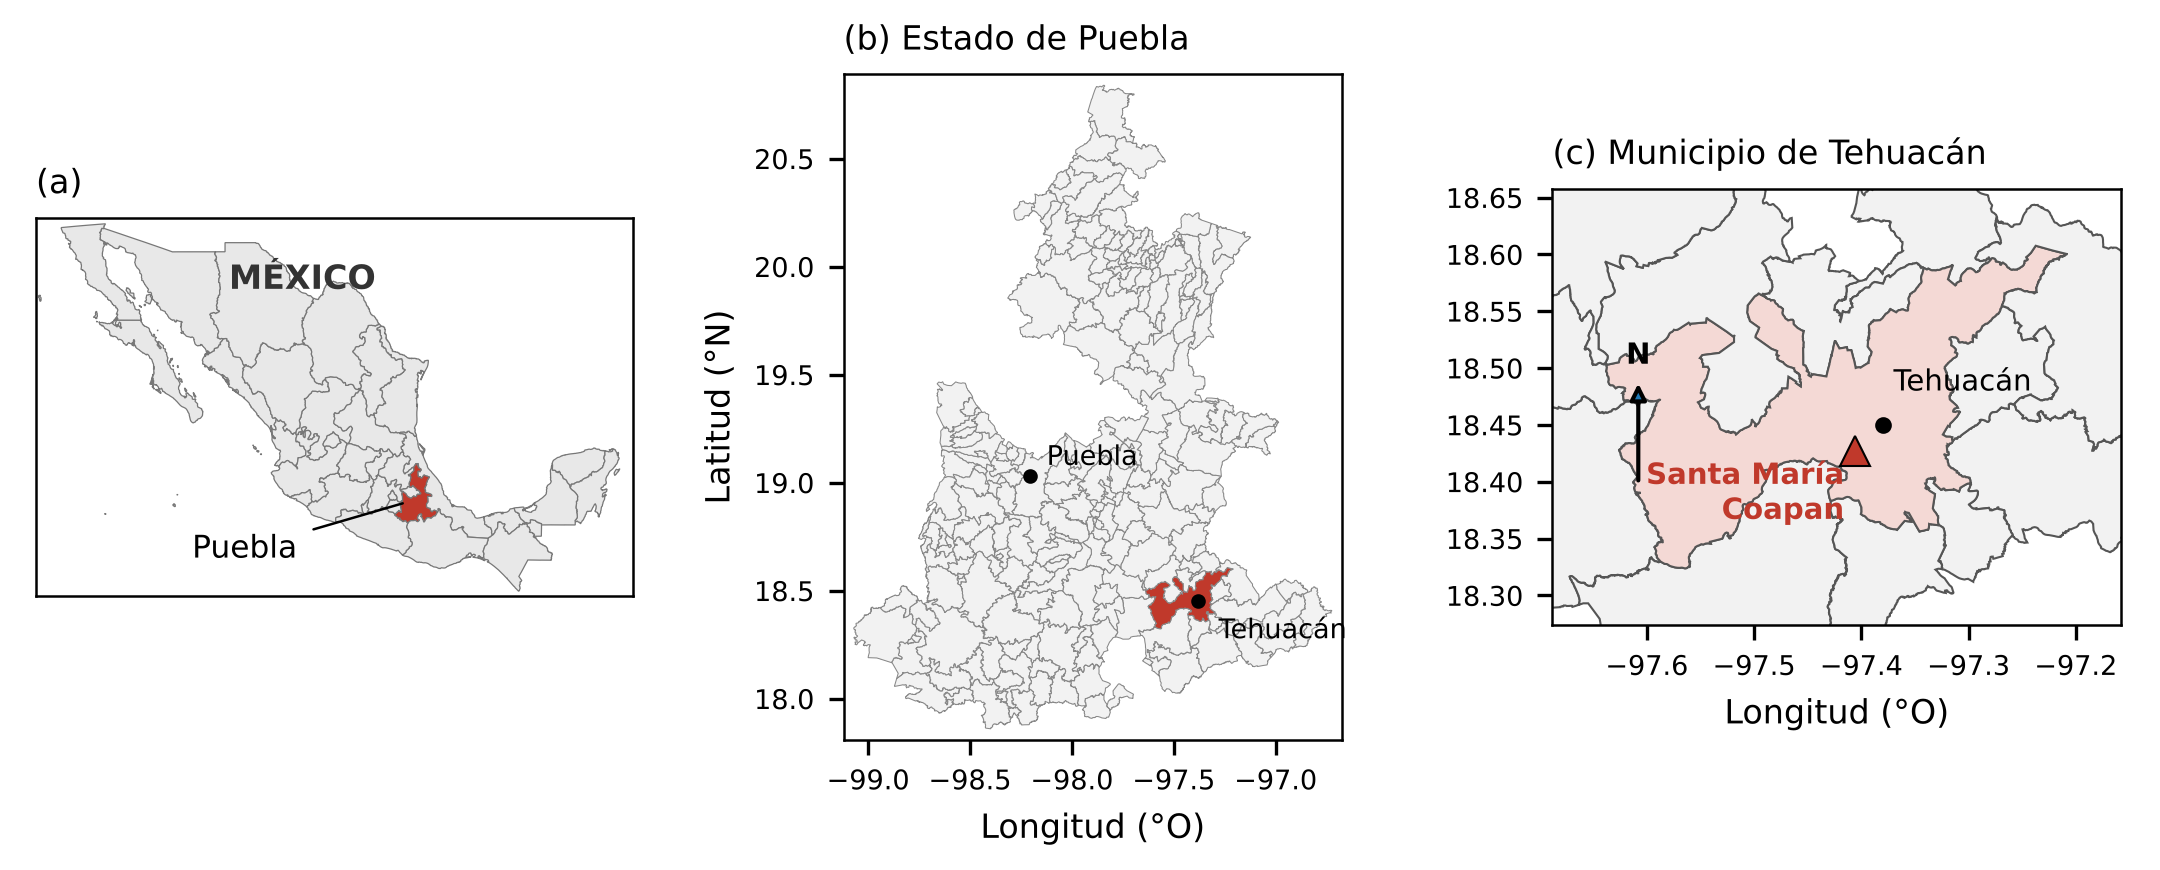
\includegraphics[width=0.92\textwidth]{f1_localizacion.png}
\caption{Localización regional del caso de estudio. (a) República Mexicana y estado de Puebla. (b) Municipios de Puebla; en rojo, Tehuacán. (c) Valle de Tehuacán, carretera federal MEX-125, iglesia de Santa María Coapan \cite{gcatholic} y ubicación del relleno sanitario. Elaboración propia con límites vectoriales abiertos \cite{natural,phantom}.}
\label{fig:loc}
\end{figure*}

\section{Localización}
Santa María Coapan es una junta auxiliar del municipio de Tehuacán, en el sureste del estado de Puebla (Fig.~\ref{fig:loc}). El relleno se ubica junto al km 12.2 de la carretera federal Tehuacán--Huajuapan (MEX-125) \cite{linares}, dentro de la subzona de aprovechamiento especial de la Reserva de la Biosfera Tehuacán--Cuicatlán \cite{publimetro,conanp}. A partir de dos coordenadas oficiales de inspección de la PROFEPA (18\textdegree24$'$12.3$''$N, 97\textdegree25$'$41.8$''$O en el acceso suroeste y 18\textdegree24$'$05.88$''$N, 97\textdegree25$'$30.03$''$O al sur-sureste) y ortoimágenes de alta resolución (24 de agosto de 2025, 0.34\,m) \cite{esri}, se delimitó el predio en coordenadas UTM Zona 14N (EPSG:32614, Fig.~\ref{fig:del}). El centroide del cuerpo principal queda en 18\textdegree24$'$17.53$''$N, 97\textdegree25$'$36.68$''$O (666,169.8\,E, 2,035,700.0\,N), a 723\,m al sureste de la carretera MEX-125, 1.79\,km al noroeste de San Andrés Arrealco, 2.08\,km al estenoreste de San Antonio Texcala, 3.33\,km al suroeste de la iglesia de Santa María Coapan (18.4274\textdegree\,N, 97.4060\textdegree\,O \cite{gcatholic}) y 7.22\,km al suroeste del centro de Tehuacán.

El sitio está en el valle de Tehuacán, una depresión tectónica limitada por fallas normales del sistema de la falla de Oaxaca, sobre depósitos cenozoicos de la Formación Tehuacán con conglomerados y capas delgadas de yeso \cite{davalos2007}. Esto importa para la interpretación: el yeso y otras sales naturales también bajan la resistividad y pueden parecerse al lixiviado. Según el Copernicus DEM GLO-30 (30\,m) \cite{esa}, el relleno está encajonado en una cabecera entre 1,751.6 y 1,814.1\,m s.n.m.\ (62.5\,m de desnivel interno, pendiente media de 12.4\textdegree\ y máxima de 28.4\textdegree), limitada al oeste por un parteaguas ($\sim$1,830\,m) y con drenaje superficial D8 hacia el este-noreste (azimut 53.5\textdegree).

\begin{figure*}[!t]
\centering
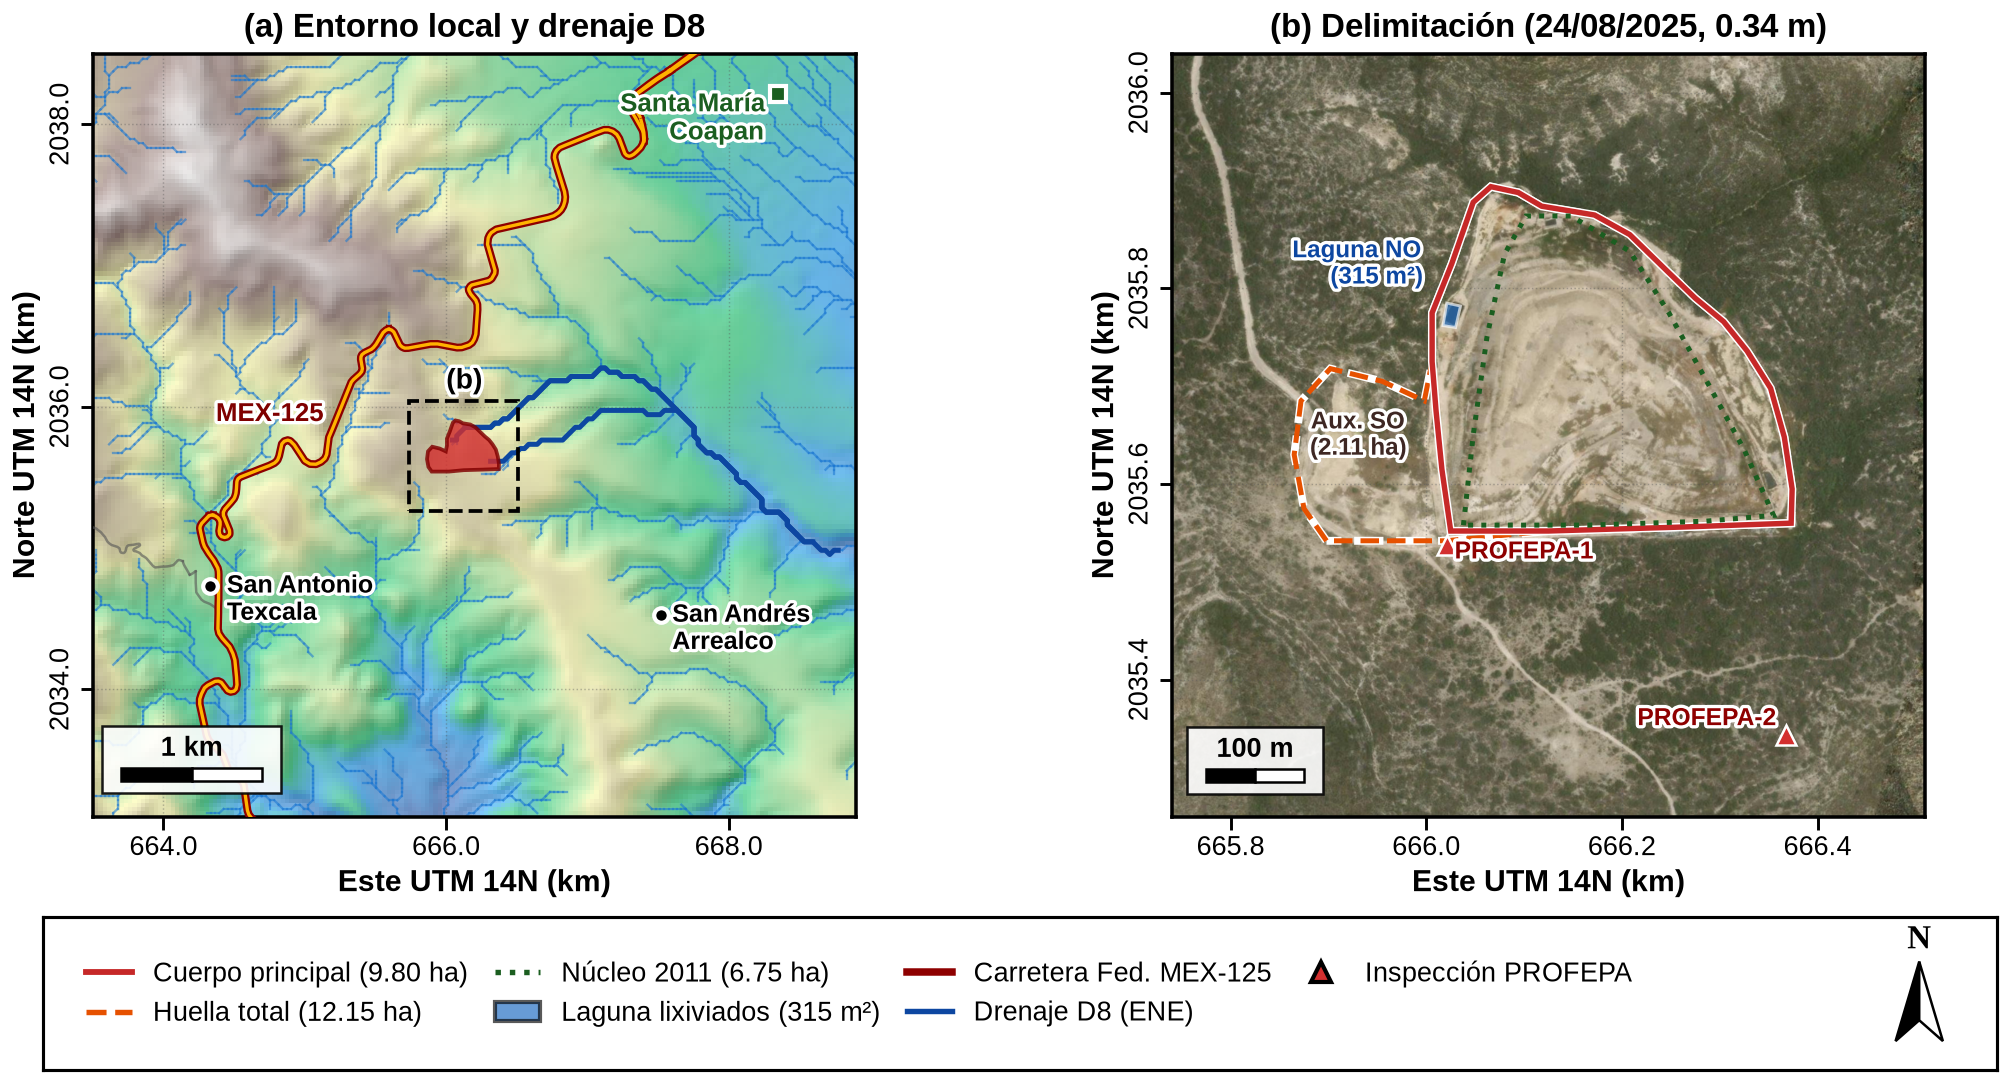
\includegraphics[width=0.92\textwidth]{f2_delimitacion.png}
\caption{Localización local y delimitación del relleno sanitario de Santa María Coapan en UTM Zona 14N (EPSG:32614). (a) Relieve (Copernicus DEM 30\,m), carretera federal MEX-125, localidades cercanas y rutas de escurrimiento D8 hacia el ENE. (b) Delimitación sobre ortoimagen de alta resolución (24/08/2025, 0.34\,m): cuerpo principal (9.80\,ha), huella operativa total (12.15\,ha), núcleo 2011 (6.75\,ha), área auxiliar SO (2.11\,ha), laguna de lixiviados NO (315\,m$^2$) y puntos de inspección PROFEPA. Elaboración propia con datos Esri Wayback \cite{esri} y ESA \cite{esa}.}
\label{fig:del}
\end{figure*}

El análisis multitemporal (1993--2025, Fig.~\ref{fig:evo}) acota el desmonte inicial entre febrero de 1993 y diciembre de 1994 \cite{usgs}, muestra una expansión de +3.05\,ha (+45.2\,\%) posterior a 2010 y revela trincheras en el sector suroeste desde 2013. Una síntesis multisensor de noviembre de 2026 sobre Sentinel-2 (03/11/2026) y SAR Sentinel-1 (19/11/2026) \cite{esa} confirma que el 87.5\,\% de la huella permanece como cubierta mineral o suelo desnudo sin vegetación (NDVI mediano de 0.112 frente a 0.329 en matorral testigo; retrodispersión VV $=-10.42$\,dB con cambio $\Delta$VV $=-1.96$\,dB desde octubre de 2021) y conserva una poza activa de lixiviados en el borde noroeste (315\,m$^2$). El acuífero regional más probable es el Valle de Tehuacán (clave 2105), donde la CONAGUA reporta niveles estáticos entre 12 y más de 110\,m según la posición en el valle \cite{dof2013,conagua}; la profundidad exacta del nivel del agua bajo el sitio falta y se medirá en los piezómetros.

\begin{figure}[!t]
\centering
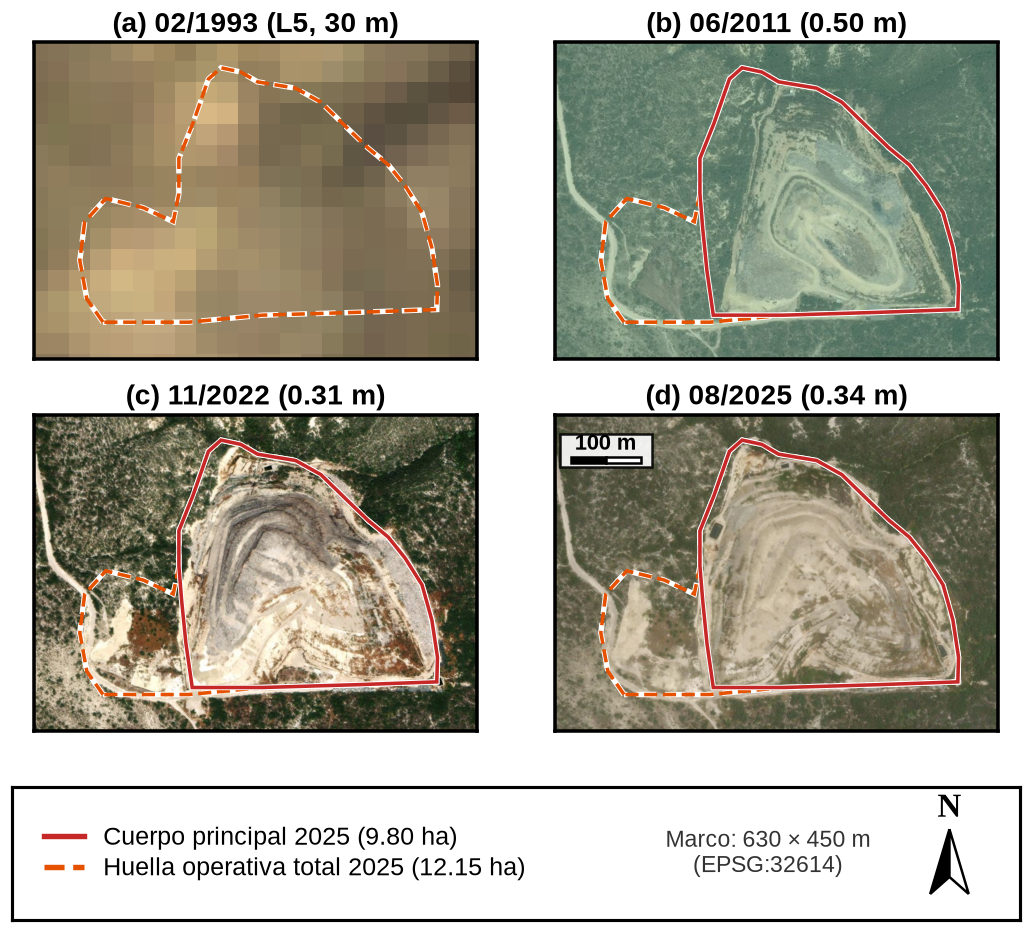
\includegraphics[width=\columnwidth]{f3_evolucion.png}
\caption{Evolución superficial del sitio entre 1993 y 2025 con la huella actual superpuesta. (a) 15/02/1993 (Landsat-5, 30\,m): terreno sin desmonte visible. (b) 06/06/2011 (0.50\,m): núcleo de 6.75\,ha tras concluir la vida útil original. (c) 18/11/2022 (0.31\,m): cicatriz oscura tras el incendio de mayo de 2022. (d) 24/08/2025 (0.34\,m): cubierta mineral sin vegetación y laguna de lixiviados NO. Elaboración propia con datos USGS Landsat C2 L2 \cite{usgs} y Esri World Imagery Wayback \cite{esri}.}
\label{fig:evo}
\end{figure}

\section{Objetivos}
\subsection{General}
Delimitar espacialmente el relleno sanitario de Santa María Coapan y proponer un levantamiento geofísico integrado para delimitar los residuos y el lixiviado, mostrando con una simulación qué se puede resolver con ese diseño.

\subsection{Específicos}
\begin{enumerate}
\item Reunir y ordenar la información pública del caso, separando hechos de afirmaciones.
\item Delimitar geoespacialmente el predio, su evolución superficial (1993--2026) y su red de escurrimiento D8 en EPSG:32614.
\item Elegir los métodos geofísicos adecuados para cada pregunta y diseñar la adquisición con extensión \emph{roll-along}.
\item Simular en 2.5D un perfil de ERT para estimar qué tan bien se recuperarían el cuerpo de residuos y el lixiviado.
\item Proponer cómo confirmar las anomalías con piezómetros, definir un plan de acción y plantear monitoreo anual.
\end{enumerate}

\section{Justificación}
La PROFEPA ordenó un estudio del daño y un plan de remediación \cite{greenpeace,profepa}, pero no hay un mapa del subsuelo que diga dónde actuar. Perforar sin guía es caro y puede pasar de largo el lixiviado. Los métodos eléctricos y electromagnéticos cubren el predio completo en pocos días, no abren el terreno y orientan dónde conviene perforar. Además, el sitio está en una subzona de aprovechamiento especial de la Reserva de la Biosfera Tehuacán--Cuicatlán \cite{publimetro,conanp}, así que saber si el lixiviado avanza hacia el área protegida tiene valor ambiental directo. Por último, el relleno debía cerrar en 2010 y siguió operando \cite{linares}; documentar el daño con datos físicos da una base técnica común a la comunidad, a las autoridades y a quien ejecute la remediación.

\section{Métodos geofísicos propuestos}
La Tabla~\ref{tab:met} resume qué método responde qué pregunta. Los valores de resistividad y cargabilidad son de otros rellenos \cite{abdulrahman2016,rawfill}; en Coapan pueden ser distintos. La ERT es el método central porque la resistividad responde directo a la salinidad del agua en el terreno. La IP se mide con los mismos equipos y electrodos, así que su costo extra es bajo. El EM cubre rápido todo el predio y decide dónde priorizar anomalías. La magnetometría se agrega por la sospecha de residuos industriales metálicos. El GPR se usa solo en tramos cortos. Ningún método basta solo, y por eso se proponen varios junto con confirmación hidroquímica directa.

\begin{table*}[!t]
\caption{Métodos geofísicos propuestos, pregunta que responden y respuesta esperada}
\label{tab:met}
\centering
\small
\begin{tabular}{@{}p{0.11\textwidth}p{0.19\textwidth}p{0.29\textwidth}p{0.29\textwidth}@{}}
\toprule
Método & Pregunta & Respuesta esperada & Limitación principal\\
\midrule
ERT & ¿Dónde están los residuos y el lixiviado, y a qué profundidad? & Residuos: 0.5 a 30\,\ohmm\ \cite{rawfill}. Lixiviado: menos de 10\,\ohmm\ \cite{abdulrahman2016}. Fondo seco: decenas de \ohmm. & Las sales naturales también bajan la resistividad. Resolución disminuye con la profundidad.\\
IP & ¿Qué tipo de material genera la anomalía? & Residuos con metales: cargabilidad alta ($>70$\,ms en un caso). Lixiviado disuelto: baja ($<20$\,ms) \cite{abdulrahman2016}. & Posible ambigüedad por carbón y cenizas del incendio de 2022; ruido mayor que en ERT.\\
EM (FDEM) & ¿Cuál es la extensión lateral de la zona conductora? & Mapa de conductividad aparente; anomalía alta sobre residuos y lixiviado somero. & Poca resolución en profundidad; muy sensible a cercas metálicas y objetos superficiales.\\
Magnetometría & ¿Hay tambores metálicos o chatarra enterrada? & Anomalías dipolares locales e intensas sobre concentraciones metálicas. & Las latas y el hierro de residuos urbanos dan ruido de fondo; alteración térmica en área quemada.\\
GPR & ¿Cuánto mide la cubierta y hay celdas o zanjas? & Reflectores someros de la cubierta y bordes de celdas o trincheras. & Se atenúa muy rápido en suelo húmedo, arcilloso o con lixiviado conductor.\\
Piezómetros y muestras & ¿La anomalía geofísica es contaminación real? & Nivel del agua, conductividad eléctrica, iones y metales pesados en agua y suelo. & Cobertura puntual y mayor costo; sirven para calibrar y confirmar, no para mapear.\\
\bottomrule
\end{tabular}
\end{table*}

\section{Diseño de adquisición de datos}
La Fig.~\ref{fig:dis} proyecta el levantamiento sobre el polígono real en EPSG:32614. Como el ancho del cuerpo principal alcanza 350--370\,m, un tendido fijo de 235\,m no cubre ambos bordes naturales. Por ello se mantiene el espaciado de electrodos de 5\,m y se amplían las líneas mediante extensión \emph{roll-along}: seis perfiles E--O (L1--L6, 275 a 435\,m, separados 55\,m) y dos transversales N--S (T1 de 395\,m y T2 de 355\,m) que se cruzan para control de consistencia, sumando 3,315\,m de ERT/IP (Tabla~\ref{tab:par} y Tabla~\ref{tab:coord}). Los perfiles L4, L5 y T1 atraviesan además la zona quemada en mayo de 2022 (2.92\,ha con índice diferencial normalizado de área quemada, \emph{differenced Normalized Burn Ratio}, dNBR $\geq$ 0.10) y el borde del estanque de lixiviados noroeste (315\,m$^2$), donde se tomará conductividad eléctrica, pH y temperatura directa del líquido superficial como referencia física.

Con base en el modelo de flujo superficial D8, el perfil de fondo R1 (235\,m, 48 electrodos) se sitúa aguas arriba al oeste sobre matorral intacto ($\sim$1,820\,m s.n.m.), evitando contaminación por escorrentía para aislar la resistividad natural de las sales y yesos del terreno. Los piezómetros quedan orientados por el gradiente topográfico hacia el ENE: P1 testigo aguas arriba al oeste y P2--P4 formando un triángulo aguas abajo en las cañadas de descarga (Tabla~\ref{tab:coord}). La malla EM y magnetométrica (28.1\,ha, 609 $\times$ 462\,m) cubre toda la huella más 50\,m de margen, incluyendo el sector auxiliar suroeste con trincheras históricas. Para hacer viable la magnetometría en laderas de 12--28\textdegree, se plantea una etapa base con líneas cada 10\,m en toda la malla y detalle cada 5\,m solo sobre el cuerpo principal y anomalías EM.

\begin{figure}[!t]
\centering
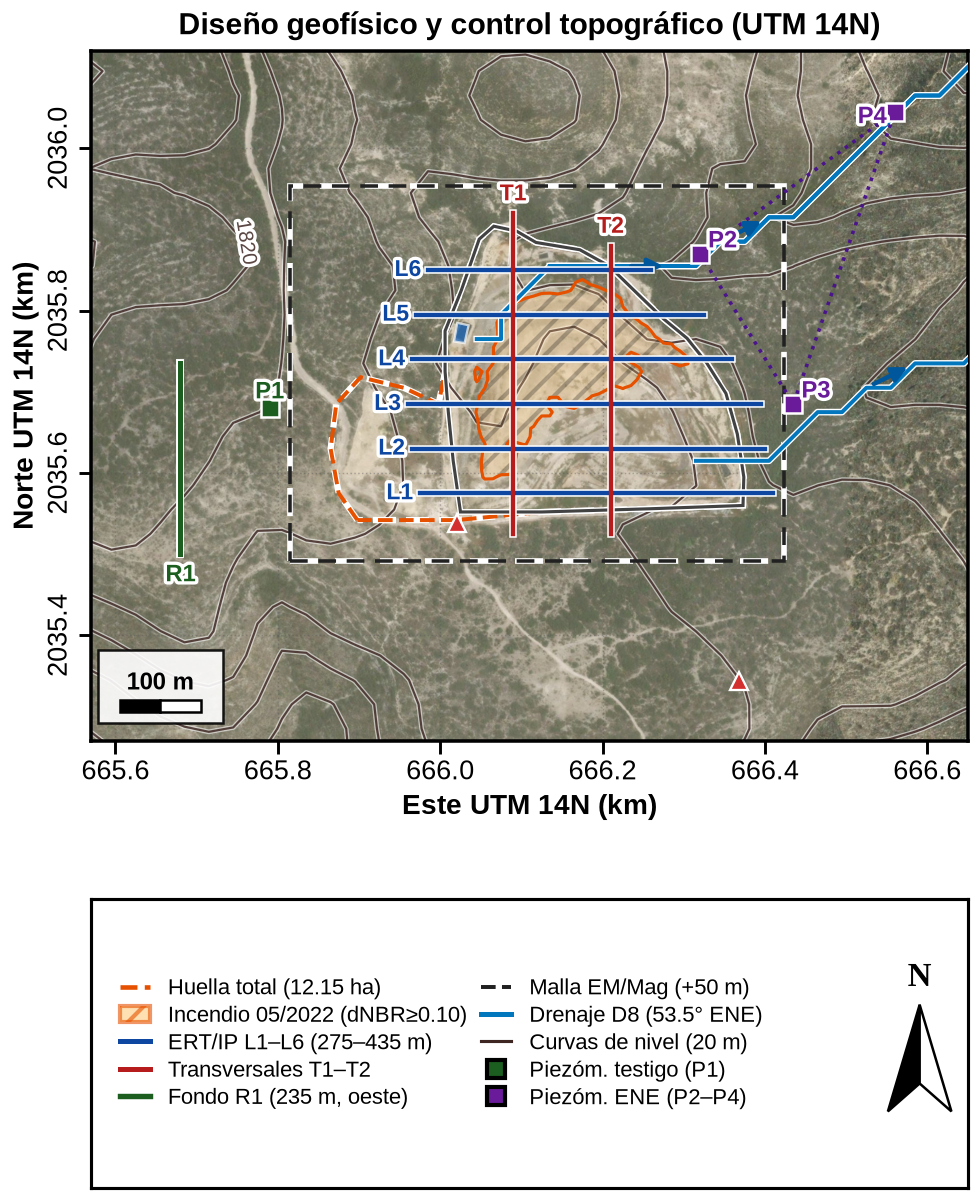
\includegraphics[width=\columnwidth]{f4_diseno.png}
\caption{Diseño de adquisición geofísica y control topográfico georreferenciado en EPSG:32614. Se integran curvas de nivel cada 20\,m (Copernicus DEM), drenaje superficial D8 hacia el ENE (azimut 53.5\textdegree), perfiles ERT/IP E--O (L1--L6, 275--435\,m con \emph{roll-along} cada 5\,m), transversales T1--T2, perfil de fondo R1 aguas arriba al oeste, malla EM/magnetométrica (+50\,m, 28.1\,ha), cicatriz del incendio de mayo de 2022 (dNBR $\geq$ 0.10) y piezómetros P1--P4. Elaboración propia.}
\label{fig:dis}
\end{figure}

Se debe medir la resistencia de contacto de cada electrodo y repetir mediciones con error mayor a 3\,\%. El levantamiento se estima en 15--18 días de campo (11--13 de ERT/IP con \emph{roll-along}, 3--4 de EM/magnetometría escalonada y 1 de GPR). Por el incendio de mayo de 2022 y los residuos peligrosos, es obligatorio inspeccionar previamente con detector multigas (CH$_4$, CO, H$_2$S, O$_2$) y cámara térmica portátil antes de hincar electrodos.

\begin{table}[!t]
\caption{Parámetros de adquisición propuestos}
\label{tab:par}
\centering
\small
\begin{tabular}{@{}p{0.23\columnwidth}p{0.65\columnwidth}@{}}
\toprule
Elemento & Parámetro propuesto\\
\midrule
ERT/IP & Electrodos cada 5\,m, arreglo Wenner--Schlumberger. 6 perfiles E--O separados 55\,m con \emph{roll-along} (L1--L3: 435\,m, L4: 395\,m, L5: 355\,m, L6: 275\,m), 2 transversales N--S (T1: 395\,m, T2: 355\,m) y fondo R1 (235\,m). Total: 3,315\,m.\\
Profundidad & $\sim$30\,m en tendido base de 235\,m (0.17 veces la apertura máxima \cite{edwards1977}) y hasta $\sim$55--70\,m en el centro de líneas \emph{roll-along} de 355--435\,m.\\
IP & Dominio del tiempo en las mismas líneas ERT; interpretar junto con dNBR para no confundir carbón/cenizas con chatarra.\\
EM (FDEM) & Estaciones cada 10\,m en líneas cada 20\,m sobre la huella total, sector auxiliar SO y 50\,m de amortiguamiento (28.1\,ha).\\
Magnetometría & Malla regional con líneas cada 10\,m (lecturas 1\,m) en 28.1\,ha, y relleno cada 5\,m sobre el cuerpo principal y anomalías EM.\\
GPR & Tramos de 50 a 100\,m sobre L2 y L5 (cubierta seca y bordes de celdas).\\
Piezómetros & 4 puntos (P1 testigo aguas arriba; P2--P4 en triángulo aguas abajo hacia el ENE según flujo D8); nivel del agua, CE, iones y metales, más muestreo directo en laguna NO.\\
Posición & GPS diferencial / RTK en electrodos y estaciones con levantamiento topográfico completo para inversión 2D con topografía.\\
\bottomrule
\end{tabular}
\end{table}

\begin{table*}[!t]
\caption{Coordenadas georreferenciadas clave del sitio y red de control (UTM Zona 14N, EPSG:32614)}
\label{tab:coord}
\centering
\small\setlength{\tabcolsep}{3pt}
\begin{tabular}{@{}llrrl@{}}
\toprule
Elemento & Función / Ubicación & Este (m) & Norte (m) & Cota (m s.n.m.) / Nota\\
\midrule
Centroide cuerpo & Centro geométrico del cuerpo principal (9.80\,ha) & 666,169.8 & 2,035,700.0 & 1,783.4 (media huella)\\
PROFEPA-1 & Acceso SO (18\textdegree24$'$12.3$''$N, 97\textdegree25$'$41.8$''$O) & 666,021.0 & 2,035,538.0 & Referencia oficial\\
PROFEPA-2 & Control SSE (18\textdegree24$'$05.88$''$N, 97\textdegree25$'$30.03$''$O) & 666,368.1 & 2,035,343.6 & Referencia oficial\\
Laguna NO & Poza activa de lixiviados (315\,m$^2$) & 666,025.7 & 2,035,772.4 & Calibración CE/pH in situ\\
Perfil R1 & Fondo testigo aguas arriba (O) & 665,680.0 & 2,035,500--2,035,735 & 235\,m ($\sim$1,820\,m s.n.m.)\\
P1 & Piezómetro testigo aguas arriba (O del camino) & 665,790.0 & 2,035,680.0 & 1818.2\,m snm\\
P2 & Aguas abajo --- salida cañada principal NE & 666,320.0 & 2,035,870.0 & 1735.6\,m snm\\
P3 & Aguas abajo --- pie de talud E hacia tributario ENE & 666,435.0 & 2,035,685.0 & 1749.7\,m snm\\
P4 & Aguas abajo --- control distal ENE rumbo a Tehuacán & 666,560.0 & 2,036,045.0 & 1696.6\,m snm\\
\bottomrule
\end{tabular}
\end{table*}

\section{Procesamiento e interpretación esperada}
\subsection{Procesamiento}
Los datos de ERT se editarán para eliminar mediciones ruidosas y se invertirán en 2D incluyendo obligatoriamente la topografía real medida a lo largo de cada perfil (desnivel interno de 62.5\,m y taludes de hasta 28.4\textdegree), con criterio de suavidad. Se reportará el ajuste (RMS) y la zona que los datos sí alcanzan a resolver para no interpretar fuera de ella \cite{loke1996}, evaluando además posibles artefactos 3D laterales en las líneas cercanas a la barranca (L5--L6). La IP se invertirá de forma lineal sobre el modelo de resistividad. El EM se interpolará a un mapa de conductividad aparente, y la magnetometría se corregirá por variación diurna antes de obtener la anomalía de campo total.

\subsection{Simulación sintética}
Para evaluar la respuesta esperada, se implementó un código propio de modelado directo en 2.5D por volúmenes finitos (cuadratura de Fourier no negativa calibrada contra semiespacio homogéneo) acoplado a una inversión suavizada de tipo Loke--Barker \cite{loke1996}. El modelo sintético utiliza valores de literatura: cubierta seca (120\,\ohmm), terreno natural (90\,\ohmm), roca basal a más de 28\,m (300\,\ohmm), un cuerpo de residuos entre 55 y 165\,m de distancia y 1.5 a 14\,m de profundidad (30\,\ohmm), una pluma de lixiviado subyacente hacia el este (115--205\,m, 14--24\,m, 6\,\ohmm) y una bolsa somera de lodos salinos de 20 por 4\,m (8\,\ohmm). Se calcularon 901 mediciones con el arreglo Wenner--Schlumberger sobre 48 electrodos cada 5\,m (235\,m), se les agregó 3\,\% de ruido gaussiano y se invirtieron sobre una malla independiente ($dx=5$\,m frente a 2.5\,m de la malla directa) para no favorecer el ajuste.

\begin{figure}[!t]
\centering
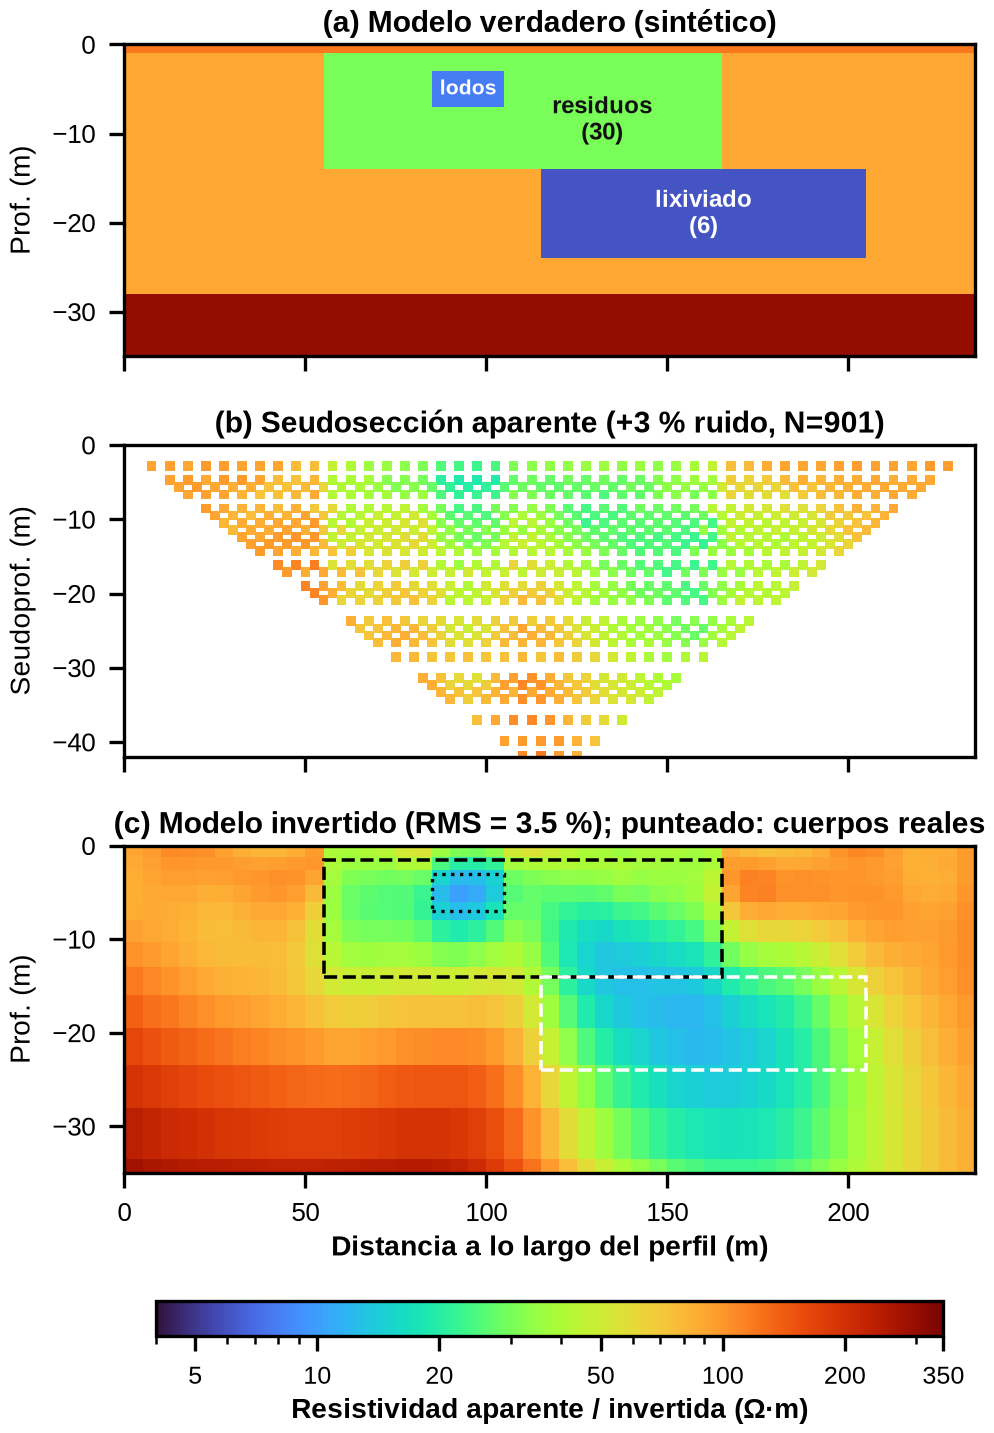
\includegraphics[width=\columnwidth]{f5_simulacion.png}
\caption{Simulación numérica 2.5D de un perfil ERT base de 48 electrodos (235\,m). (a) Modelo verdadero sintético. (b) Seudosección de resistividad aparente simulada con 3\,\% de ruido (901 datos Wenner--Schlumberger). (c) Modelo invertido en malla independiente (RMS = 3.5\,\%); los contornos punteados marcan los cuerpos del modelo verdadero. Elaboración propia.}
\label{fig:sim}
\end{figure}

\begin{table}[!t]
\caption{Recuperación de los cuerpos en la simulación (mediana del modelo invertido)}
\label{tab:rec}
\centering
\small\setlength{\tabcolsep}{4pt}
\begin{tabular}{@{}lcc@{}}
\toprule
Zona del modelo & Verdadero (\ohmm) & Invertido (\ohmm)\\
\midrule
Residuos (1.5--14\,m) & 30 & 28\\
Lixiviado (14--24\,m) & 6 & 17\\
Bolsa de lodos (3--7\,m) & 8 & 13\\
Terreno natural, borde & 90 & 87\\
Debajo del lixiviado (26--35\,m) & 90 & 22\\
Roca basal ($>28$\,m, centro) & 300 & 88\\
\bottomrule
\end{tabular}
\end{table}

\subsection{Lectura de la simulación}
La inversión ajustó los datos con un RMS de 3.5\,\% y recuperó adecuadamente las anomalías principales (Fig.~\ref{fig:sim}, Tabla~\ref{tab:rec}). El cuerpo de residuos quedó en su posición y muy próximo al valor verdadero (28 contra 30\,\ohmm), al igual que el terreno natural en borde (87 contra 90\,\ohmm). Sin embargo, el lixiviado muestra tres limitaciones físicas que deben considerarse al leer perfiles reales:
\begin{itemize}
\item La resistividad recuperada resulta mayor (17 contra 6\,\ohmm), porque la regularización suaviza los contrastes bruscos.
\item La zona conductora se prolonga hacia abajo: entre 26 y 35\,m el modelo invertido arroja 22\,\ohmm\ donde el medio vale 90\,\ohmm; un lixiviado real no debe declararse profundo solo por ese borde de baja sensibilidad.
\item La bolsa de lodos (20 $\times$ 4\,m, 13 contra 8\,\ohmm) aparece parcialmente diluida dentro de la masa de residuos y la roca basal (300\,\ohmm) resulta atenuada (88\,\ohmm) por canalización de corriente en el conductor superior.
\end{itemize}
Esta simulación representa un tendido simple de 235\,m; con la extensión \emph{roll-along} a 355--435\,m propuesta para la zona central, aumentará la sensibilidad en profundidad ($\sim$55--70\,m), aunque persistirán el suavizado de contrastes y la necesidad de cruzar IP con el mapa dNBR del incendio de 2022.

\subsection{Cómo se interpretará con datos reales}
Se propone una regla operativa de tres condiciones: una anomalía se designará probable lixiviado únicamente si (1) presenta resistividad inferior al valor de fondo medido en \emph{R1} (con 10\,\ohmm\ como guía \cite{abdulrahman2016}, calibrada contra la conductividad medida en la laguna NO), (2) muestra continuidad espacial en cruces de perfiles \emph{L--T}, y (3) coincide con una conductividad eléctrica elevada en el piezómetro cercano. Los cuerpos de alta cargabilidad en IP se contrastarán con magnetometría y la cicatriz dNBR antes de asociarse a metales; ninguna anomalía se presentará como contaminación comprobada sin validación hidroquímica.

\section{Impacto ambiental y plan de acción}
\subsection{Impacto esperado}
El impacto se divide entre lo documentado y lo que resta comprobar en campo. Consta oficialmente que el relleno fue clausurado y que no se ha hecho público el estudio de remediación exigido \cite{greenpeace,profepa}. El análisis D8 muestra que el escurrimiento superficial converge hacia el ENE (azimut 53.5\textdegree), rumbo al valle de Tehuacán, por lo que la vigilancia hidrológica prioritaria corresponde a ese eje en dirección general hacia Santa María Coapan (3.33\,km al NE), mientras San Antonio Texcala (2.08\,km al OSO) queda separado por el parteaguas occidental y San Andrés Arrealco (1.79\,km al SE) se sitúa fuera del eje principal. Queda por verificar si existe migración hacia el acuífero 2105, alcance hacia la reserva o presencia de metales en suelo y agua.

\subsection{Plan de acción}
\begin{enumerate}
\item \textbf{Preparación y seguridad (semanas 1--2).} Validar con RTK en campo los vértices delimitados (9.80/12.15\,ha), gestionar permisos municipales y comunitarios y ejecutar inspección térmica y multigas sobre la cicatriz de 2022.
\item \textbf{Adquisición geofísica (semanas 3--5).} Medir la malla EM y magnetométrica escalonada (28.1\,ha), seguida de los 3,315\,m de perfiles ERT/IP con \emph{roll-along} y tramos GPR (Tabla~\ref{tab:par}).
\item \textbf{Procesamiento (semanas 6--7).} Invertir con topografía real, mapear anomalías y aplicar la regla de tres condiciones para seleccionar los puntos de perforación.
\item \textbf{Confirmación directa (semanas 8--9).} Perforar piezómetros \emph{P1--P4}, medir nivel del agua y tomar muestras de agua, suelo y laguna NO (CE, pH, iones mayores y metales) para contrastarlas con las secciones invertidas.
\item \textbf{Modelo conceptual y riesgo.} Integrar todo en un modelo 3D (volumen de residuos, geometría del lixiviado y dirección del flujo) como base técnica del estudio de daño requerido por la PROFEPA.
\item \textbf{Remediación y monitoreo.} Retirar residuos peligrosos y RPBI a sitios autorizados, construir cobertura final y drenaje conforme a la NOM-083-SEMARNAT-2003 \cite{nom083} y repetir anualmente la ERT en las mismas líneas de control \cite{helene2020}.
\end{enumerate}

La comunidad nahua de Santa María Coapan debe participar desde la planeación y recibir los resultados íntegros, por habitar junto al sitio y haber promovido su defensa legal; la responsabilidad de ejecutar la remediación corresponde al gobierno municipal de Tehuacán conforme a la resolución vigente \cite{greenpeace,profepa}.

\section{Conclusiones}
\begin{itemize}
\item El relleno sanitario de Santa María Coapan es un caso ambiental real en Puebla con clausura definitiva ordenada y sin estudio público del daño ni caracterización del subsuelo.
\item Una combinación georreferenciada de EM y magnetometría escalonada (28.1\,ha), 3,315\,m de ERT/IP \emph{roll-along}, GPR y cuatro piezómetros permite delimitar residuos, rutas de lixiviado y chatarra enterrada; la ERT actúa como método central.
\item La simulación 2.5D en malla independiente (RMS = 3.5\,\%) muestra que un tendido base recupera bien la geometría y resistividad de los residuos (28 contra 30\,\ohmm), aunque sobreestima la resistividad del lixiviado (17 contra 6\,\ohmm) y lo suaviza hacia abajo, limitación parcialmente compensada mediante extensión \emph{roll-along} a 355--435\,m.
\item Las sales y yesos naturales del valle de Tehuacán pueden imitar la firma del lixiviado; por ello son indispensables el perfil testigo R1 aguas arriba al oeste, la medición in situ en la laguna NO y el muestreo en P1--P4.
\item Aunque este trabajo no cuenta aún con mediciones geofísicas de campo, la ubicación real (18\textdegree24$'$17.53$''$N, 97\textdegree25$'$36.68$''$O), la delimitación multiescala (9.80\,ha principales y 12.15\,ha totales), la evolución satelital (1993--2025), la cicatriz de incendio (2.92\,ha) y el escurrimiento D8 hacia el ENE quedaron documentados en EPSG:32614, dejando el levantamiento listo para ejecutarse sin etapa exploratoria ciega.
\end{itemize}

\begin{thebibliography}{99}
\bibitem{greenpeace} Greenpeace México, ``Crisis ambiental y de derechos humanos en Tehuacán, Puebla: Greenpeace y comunidad nahua de Santa María Coapan protestan por basurero tóxico y su falta de remediación,'' comunicado de prensa. Disponible: https://www.greenpeace.org/mexico/
\bibitem{linares} A. Linares Déctor, ``El relleno sanitario de Tehuacán, Puebla: un estudio sociológico de la crisis del manejo de residuos, 2015--2022,'' tesis, Benemérita Univ. Autónoma de Puebla. Disponible: https://repositorioinstitucional.buap.mx/
\bibitem{ciudadano} ``Incendio borra pruebas de que basurero en Coapan opera como tiradero tóxico: Comité de Bienes,'' \textit{El Ciudadano}, 13 de mayo de 2022. Disponible: https://www.elciudadano.com/
\bibitem{publimetro} ``Cierre definitivo: relleno sanitario de Tehuacán es clausurado después de 25 años,'' \textit{Publimetro}, 13 de junio de 2022. Disponible: https://www.publimetro.com.mx/puebla/
\bibitem{desinformemonos} Comunicado ``Protesta ante PROFEPA: basureros de Tehuacán y Cholula,'' \textit{Desinformémonos}, 17 de julio de 2024. Disponible: https://desinformemonos.org/
\bibitem{gcatholic} GCatholic.org, ``Iglesia Santa María de la Asunción, Santa María Coapan, Puebla,'' Plus Code 76C4CHGV+XJ. Disponible: https://gcatholic.org/churches/mexico/66183
\bibitem{davalos2007} O. G. Dávalos-Álvarez, Á. F. Nieto-Samaniego, S. A. Alaniz-Álvarez, E. Martínez-Hernández y E. Ramírez-Arriaga, ``Estratigrafía cenozoica de la región de Tehuacán y su relación con el sector norte de la falla de Oaxaca,'' \textit{Rev. Mex. Cienc. Geol.}, vol. 24, n.\textsuperscript{o} 2, pp. 197--215, 2007.
\bibitem{dof2013} Comisión Nacional del Agua, ``Acuerdo por el que se actualiza la disponibilidad media anual de agua en acuíferos, incluido el Valle de Tehuacán (clave 2105),'' \textit{Diario Oficial de la Federación}, 5 de diciembre de 2013.
\bibitem{abdulrahman2016} A. Abdulrahman \textit{et al.}, ``Characterization of active and closed landfill sites using 2D resistivity/IP imaging: case studies in Penang, Malaysia,'' \textit{Environ. Earth Sci.}, vol. 75, art. 347, 2016, doi:10.1007/s12665-015-5003-5.
\bibitem{maurya2017} P. K. Maurya \textit{et al.}, ``Detailed landfill leachate plume mapping using 2D and 3D electrical resistivity tomography with correlation to ionic strength measured in screens,'' \textit{J. Appl. Geophys.}, vol. 138, pp. 1--8, 2017.
\bibitem{helene2020} L. P. I. Helene, C. A. Moreira y R. C. Bovi, ``Identification of leachate infiltration and its flow pathway in landfill by means of electrical resistivity tomography (ERT),'' \textit{Environ. Monit. Assess.}, vol. 192, 2020, doi:10.1007/s10661-020-8206-5.
\bibitem{rawfill} RAWFILL, ``SWOT analysis of geophysical methods for landfill characterisation,'' Interreg NWE, informe técnico. Disponible: https://vb.nweurope.eu/
\bibitem{edwards1977} L. S. Edwards, ``A modified pseudosection for resistivity and IP,'' \textit{Geophysics}, vol. 42, n.\textsuperscript{o} 5, pp. 1020--1036, 1977.
\bibitem{loke1996} M. H. Loke y R. D. Barker, ``Rapid least-squares inversion of apparent resistivity pseudosections using a quasi-Newton method,'' \textit{Geophys. Prospect.}, vol. 44, n.\textsuperscript{o} 1, pp. 131--152, 1996.
\bibitem{nom083} Secretaría de Medio Ambiente y Recursos Naturales, ``NOM-083-SEMARNAT-2003: Especificaciones de protección ambiental para la selección del sitio, diseño, construcción, operación, monitoreo, clausura y obras complementarias de un sitio de disposición final de residuos sólidos urbanos y de manejo especial,'' \textit{Diario Oficial de la Federación}, 2004.
\bibitem{natural} Natural Earth, ``Admin 1 -- States, Provinces,'' conjunto de datos vectoriales, dominio público. Disponible: https://www.naturalearthdata.com/
\bibitem{phantom} PhantomInsights, ``mexico-geojson: límites municipales de México (2020),'' repositorio de GitHub. Disponible: https://github.com/PhantomInsights/mexico-geojson
\bibitem{conanp} CONANP, ``Acuerdo por el que se da a conocer el Resumen del Programa de Manejo de la Reserva de la Biosfera Tehuacán-Cuicatlán,'' \textit{Diario Oficial de la Federación}, México (Subzona de Aprovechamiento Especial, 16.46439\,ha en relleno sanitario de Tehuacán).
\bibitem{conagua} Comisión Nacional del Agua, ``Actualización de la disponibilidad media anual de agua en el acuífero Valle de Tehuacán (2105), Estado de Puebla,'' Subdirección General Técnica, CONAGUA, México.
\bibitem{profepa} PROFEPA, Resolución Administrativa PFPA/03.2/2C27.1/0036/23/0059 (Expediente PFPA/3.2/2C.27.1/00036-20), clausura total y definitiva del sitio de disposición final en Santa María Coapan, 27 de junio de 2023.
\bibitem{usgs} U.S. Geological Survey, ``Landsat Collection 2 Level-2 Surface Reflectance (LT04, LT05, LC08, Path 025/Row 047),'' USGS / Microsoft Planetary Computer STAC, 1989--2015.
\bibitem{esa} European Space Agency, ``Copernicus Sentinel-2 L2A (T14QPF), Sentinel-1 RTC y Copernicus DEM GLO-30,'' ESA / Microsoft Planetary Computer STAC, 2020--2026.
\bibitem{esri} Esri, ``World Imagery Wayback Archive (capturas 2011--2025 verificadas vía SRC\_DATE2),'' Esri, Redlands, CA, 2025.
\end{thebibliography}

\end{document}
